
\begin{enumerate}
    \item Three glass cylinders of equal height \( H = 30 \) cm and same refractive index \( n=1.5 \) are placed on a horizontal surface as shown in figure. Cylinder I has a flat top, cylinder II has a convex top and cylinder III has a concave top. The radii of curvature of the two curved tops are the same \( (R = 3 \) m). If \( H_1, H_2, \) and \( H_3 \) are the apparent depths of a point X on the bottom of the three cylinders, respectively, the correct statement(s) is/are:
        \begin{center}
            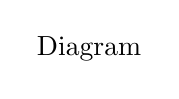
\begin{tikzpicture}
                \node {Diagram};
            \end{tikzpicture}
        \end{center}
        \begin{tasks}(2)
            \task \( H_2 \geq H_1 \)
            \task \( H_3 > H_1 \)
            \task \( H_2 > H_3 \)
            \task \( 0.8 \text{ cm} < (H_2 - H_1) < 0.9 \text{ cm} \)
        \end{tasks}
\end{enumerate}
